\subsection{Long-range number-units}
To successfully perform the NA-task, the LSTM network should encode and store the grammatical number of the subject up to one step before the verb, when prediction of the verb form (singular or plural) occurs. In some cases, this may be quite challenging, in particular in the case of a long-range dependency between subject and verb, and when another noun with an opposite number appears before the verb (cite). This section explores the underlying mechanism that enables the network to encode and store number information in various syntactic constructions, including ones with an interfering noun, and has the following structure: subsection 5.1.1 describes an ablation study, which reveals \textit{long-range number units (LR-number units)} that can store and carry number information from subject to verb, also across interfering nouns. Subsection 5.1.2 describes the intricate gate and state dynamics of LR-number units during the processing of sentences with long-range dependencies. Section 5.1.3 describes other number units that encode grammatical number for only short-range dependencies, such as in the case of a verb immediately following a subject. Finally, subsection 5.1.4 characterizes the structure of the efferent weights of number units, which propagate number information to the output layer.

\subsubsection{Local vs. distributed code - an ablation study}
Generally, number information may be stored in the network in either a local, sparse, or a distributed way, depending on the fraction of active units that carry number information. We hypothesized that if the network uses a local or sparse coding, meaning that there's a small set of units that encode number information, then ablating these units would lead to a drastic decrease in performance on the NA-task, compared to when ablating other units. To test this, we conducted ablation experiments in which each time a single unit of the network is ablated and the resulting model is then evaluated on several NA-tasks. Each NA-task contained sentences with a fixed syntactic structure, such as "Det Noun Adv Verb" or "Det Noun P Det Noun Verb", and each task was composed of several conditions depending on the possible assignments of grammatical number to the nonu(s) in the sentence (see section 3.1 for details about all NA-tasks). In addition, we also evaluated each ablated model on the Linzen task (cite). Tables 1 summarizes the results from all ablation experiments, showing units whose ablation resulted in a performance decrease of more than 10\% (TODO: choose a non-arbitrary threshold by looking at the distribution). For each NA-task, the performance of the full, non-ablated, model is also reported.


\begin{center}
\begin{table}[ht]
\begin{tabular}{|P{1.4cm}|P{0.4cm}||P{0.6cm}|P{0.6cm}|P{0.6cm}|P{0.6cm}|P{0.6cm}|P{0.6cm}|P{0.6cm}|P{0.6cm}|P{0.6cm}|P{0.6cm}|P{0.6cm}|P{0.6cm}||P{0.6cm}|}
\hline
\B NA task & \B C & \B \textcolor{blue}{770} & \B \textcolor{blue}{776} & \B \textcolor{red}{988} & \B \textcolor{red}{1283} & \B Full \\
\hline
\hline

% Singular condition

\B Simple & \B S & - &  - &    - &  - &  100 \\

\B Adv & \B S &  - &  - &  - &  - &  100 \\

\B 2Adv & \B S &  - &  - &  - &  - &  99.8 \\

\B Co-Adv & \B S &  - &  - &  \textcolor{red}{84.0} &  \textcolor{red}{84.0} &  98.8 \\

\B namePP & \B S &  - &  - &  - &  - &  98.9 \\

\B nounPP & \B SS &  - &  - & - &  - &  97.5 \\

\B nounPP & \B SP &  \B - &  - &  \textcolor{red}{58.8} &  - &  88.5 \\

\B subjrel & \B SS &   - &  - & \textcolor{red}{88.0} &  - &  97.0 \\

\B subjrel & \B SP &  \B - &  - &  - &  - &  58.8 \\

\B objrel & \B SS & \B - &  - &  - &  - &  64.7 \\

\B objrel & \B SP &  \B - &  - &  - &  - &  45.7 \\

\hline
% % Plural condition
\B Simple & \B P &  - &  - &  - &  - &  100 \\

\B Adv & \B P &  - &  - &  - &  - &  99.6 \\

\B 2Adv & \B P & - &  - & - & - &  99 \\

\B Co-Adv & \B P &  - &  \textcolor{blue}{78.9} & - &  - &  99.7 \\

\B namePP & \B P & - &  \textcolor{blue}{57.6} &  - &  - &  66.8 \\

\B nounPP & \B PS &  \textcolor{blue}{85.2} &  \textcolor{blue}{49.7} & - &  - &  93.2 \\

\B nounPP & \B PP &  - &  \textcolor{blue}{81.7} &  - &  - &  98.3 \\

\B subjrel & \B PS &  \textcolor{blue}{85.8}  &  \textcolor{blue}{58.6}  &  - &  - &  87.8 \\

\B subjrel & \B PP &  - &  \textcolor{blue}{88.1} &  - &  - &  99.3 \\

\B objrel & \B PS & - &  - &  - &  - &  69.0 \\

\B objrel & \B PP &  - &  - &  - &  - &  81.0 \\
\hline
\hline
\B Linzen & \B - &  ? &  ? &  ? &  ? &  ? \\
\hline
\end{tabular}
\caption{Ablation experiments results: Percentage of correct subject-verb agreements in all NA-tasks (section 3.1). Full - non-ablated model, C - condition, S - singular, P - plural. For task with two nouns, SS - singular-singular, SP - singular-plural, PS - plural-singular, PP - plural-plural. Red: singluar number units, Blue: Plural number units.}
\end{table}
\end{center}

We first highlight several aspects of the behavioral results of the full network (table 1 - right column) before describing in more details the ablation results. First, some NA-tasks and conditions are clearly more difficult for the network than others. For example, performance on the simple NA-task is better than that on the nounPP NA-task, which in turn is better than that of the objrel task. This matches previously reported results in humans and LSTM-LMs (cite). Second, having an interfering noun before the verb, with an opposite number than that of the subject, is clearly a more challenging task for the network - we find that for the nounPP, subjrel and objrel tasks: $ACC_{SP}>ACC_{SS}$ and $ACC_{PS}>ACC_{PP}$. We return to this point in section 5.4. Finally, for long-range dependencies, reliably encoding that the subject is singular is in most cases more difficult than plural. For example, in all the above tasks: $ACC_{SS}<ACC_{PP}$ and $ACC_{SP}<ACC_{PS}$. Interestingly, this singular-plural asymmetry has been reported also in humans (cite). We elaborate on this point in the discussion section.

We next describe several important aspects of the ablation-experiment results. First, in all NA-tasks, only four units from the entire network (1300 LSTM units in total) had a significant effect on task performance. This result suggests a local coding scheme for long-range grammatical-number information (TODO: quantify a 'significant' reduction, and perhaps link to the emergence of local coding in neural-network simulations (Bowers) and to findings about grandmother neurons in humans (e.g., Fried)). Second, we note that all number units emerged at the second layer of the network. This seems appropriate if number information needs to be directly projected to the output layer for correct verb-form prediction. In section 5.1.4 we further explore the projection weights from number units. Third, for simple, 1Adv and 2Adv NA-tasks, none of the units had a significant effect on task performance. This suggests that for short-range dependencies number information may be also encoded elsewhere in the network, perhaps via a more distributed code. We therefore make a distinction between long-range (LR) and short-range (SR) number units in what follows. We return to this point in section 5.1.3 (TODO: complete the identification of short-range number units from the resulting weights of the classifier in the generalization-across-time experiment). Fourth, LR-number units can be further divided into two types, depending on the grammatical number of the subject. Units 770 and 776 had a significant effect only when the first noun was plural, but not singular, and vice versa for units 988 and 1283 (blue and red in table 1, respectively). We therefore refer to the former as \textit{plural units} and to the latter as \textit{singular units}. Finally, we note that two of the number units (776 \& 988) had an exceptional effect on network performance in both nounPP-SP\&PS conditions. These two conditions are in particular revealing since they involve both a long-range dependency (over a prepositional phrase) and an interfering noun before the verb, while performance of the non-ablated network is still relatively high (88.5\%\&93.2\%, respectively) in contrast to these conditions in subjrel and objrel. Ablating one of these two units brought the network from high performance on the NA-task to around chance-level performance (58.8\%\&49.7\%, respectively). In the next section, we therefore focus on these two units when exemplifying gate and state dynamics of number units. 

\subsubsection{Visualizing gate and cell-state dynamics}
Results from the ablation study suggest that there's a small set of units that encodes number information for long-range dependencies, in particular, we find that in some conditions two units can bring the network from relatively high performance to around chance-level performance on the NA-task (section 5.1.1). However, it remains unclear what is the exact mechanism underlying successful trials in the NA-task, and what goes wrong in unsuccessful ones. To better understand this, we now looks into gate and state dynamics of these units during the processing of sentences from the nounPP NA-task. 

To anticipate the results and facilitate their interpretations, we begin by discussing what could be a solution to the NA-task implemented by number units in their gate and state activity. We recall that the update rule of the LSTM cell has two terms (equation 1.x). In the first term $f_t * C_{t-1}$, the forget gate controls whether to keep the previous content $C_{t-1}$ stored in the cell ($f_t=1$ - perfect remembering), or forget it ($f_t=0$ - complete forgetting). In the second term $i_t*\tilde{C}_t$, the input gate controls whether the information currently presented to the network could be updated onto the cell state: $i_t=1$ - full access, $i_t=0$ - no access. Therefore, to produce correct number agreement, it seems that number units should at least have the following three properties: (1) The grammatical number of the subject should first be encoded by $\tilde{C}_{t_{subject}}$, encoding singular and plural with \textit{different} values. (2) To grant the encoded grammatical number $\tilde{C}_{t_{subject}}$ access to the cell, the input gate should be open at the time when the subject is presented: $i_{t_{subject}}>0$, and ideally $i_{t_{subject}}=1$. In addition, to protect the stored grammatical number from interfering information updating onto the cell, such as in the case of an interfering noun, the input gate should be closed during all successive time steps until the verb: $i_t=0, t<t_{verb}$; (3) Finally, to successfully store number information in the cell for a long-range dependency, the forget gate should be in a remembering state, starting one time step after the subject: $f_t=1, t>t_{subject}$. In addition, to clean up the cell from previously stored information, the forget gate should reset when the subject is presented: $f_{t_{subject}}=0$. Figure 1B summarizes these three presumably desired properties.

Figure 2 presents the actual gate and state dynamics of units 776 and 988 during the processing of sentences from the nounPP NA-task. For each unit, we draw the dynamics of the suggestion $\tilde{C}_t$ (panels A-B), input-gate (panels C-D), forget-gate (panels E-F) and the cell variable (G-H). For each of these cases, the four condition (SS, SP, PS and PP) are described in separate curves. Error-bars represent standard deviation across 1000 sentences in each condition.

\begin{figure*}[ht]
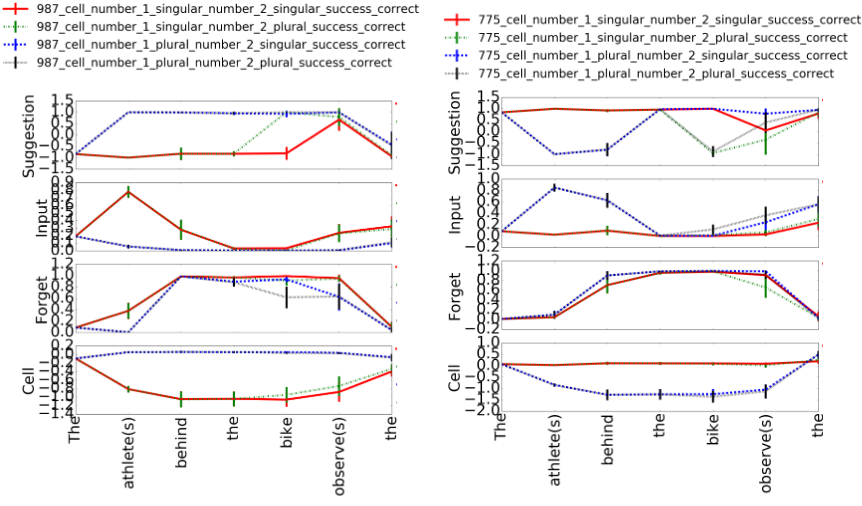
\includegraphics[width=\textwidth]{Figures/Figure2_number_units_775_987.png}
\caption{Cell and gate activations during processing of a sentence with a prepositional phrase between subject and verb. (A) Cell activity $C_t$ for the two number units 775 and 987 and output activity $h_t$ for the syntax unit 1149, for all four combinations of grammatical numbers of the two nouns. Note that the cell activity of units 775/987 is non-zero only when the first noun is plural/singular, respectively. (B) Corresponding forget-gate activity for the same number units. Note that gate activity is indifferent of the grammatical number of both nouns and that its value is close to one during the PP until after the verb. (C) Input-gate activity of the same units. Note that the gate value of unit 775/987 spikes around the first noun only when it is plural/singular.}
\end{figure*}


We describe the results along the order of the properties discussed above. First, the values of the cell suggestions $\tilde{C_t}$ of both units seem to obey the first property. For the singular unit 988, we find that singular nouns are encoded with negative values $\tilde{C}_{t_{subject}}~=-1$, and plurals with positive $\tilde{C}_{t_{subject}}~=1$ (panel A), and similarly for unit 776 (panel B). This shows that singular and plural nouns are indeed encoded differently by these units, in accordance with the results of the ablation study that suggested the labeling of units 988 and 776 as singular and plural units, respectively.

Second, input-gate dynamics of both number units seem to correspond to the second property described above. Input-gate activity spikes around the subject and stays approximately zero for subsequent time steps until the verb. One difference with respect to the desired property is the non-zero activity of the input gate at the time step immediately following the subject. This may be due to various reasons and requires further research. One possible explanation for this is that the network has developed this behavior as a heuristic to deal with compound nouns, given that for compound nouns the relevant number information resides at the second noun, whereas in the case of simple nouns there's anyway no risk of encountering an interfering noun immediately after the subject (TODO: discuss this part in the meeting to see if it makes sense to all. If yes, perhaps we could easily check this in an experiment.). Finally, note that for unit 988, the input gate is only open when the subject is singular, whereas for unit 776 it is only open when the subject is plural. This too is consistent with the labeling of these units as singular and plural.

Third, forget-gate dynamics of both number units also seem to correspond to the above properties. In both units, forget-gate activity starts at value around zero $f_{t_{subject}~=0}$ and then goes abruptly towards its maximal value at the next step $t_{subject}+1$, then stably staying at this level until after the verb $t_{verb}+1$. Note that for all four conditions (SS, SP, PS and PP), the forget-gate exhibits similar dynamics, being indifferent to the grammatical number of the subject. This seems appropriate for whether the second noun is singular or plural given that the network cannot know in advance whether an interfering noun will appear, and it should anyway store number information for long-range dependencies also in the absence of any upcoming noun (TODO: explain or leave as an open question the reason for which we observe the same dynamics whether the first noun is singular or plural). Last, we note that in all cases the forget-gate activity resets at $t_{verb}+1$. This seems appropriate, given that at this point the subject's number is no more useful, and the cell would be better free up to encode new number information.
 
Finally, cell activity should reflect the dynamics of the suggestion, input and forget gates. Indeed, the cell value becomes non-zero at $t_{subject}$ and preserves this value until $t_{verb}-1$ when verb-form prediction occurs (Panels G-H). Note that this is the case only for the relevant conditions: in conditions SS and SP, unit 987 encodes singular as $C_t ~= -1$ and is approximately zero during sentence processing in the other two conditions (PP and PS). Similarly, unit 776 encodes plural with a non-zero, negative, value only in the relevant conditions (PP and PS) but not in the irrelevant ones (SS and SP). Note that for the irrelevant conditions, cell activity is kept approximately zero thanks to the clear-up of the cell: $f_{t_{subject}}=0$ and $i_{t_{subject}}=0$, and the following input- and forget-gate dynamics.

Taken together, these results describe the intricate mechanism underlying subject-verb agreement in LSTM number units. They also clarify why ablating either one of these two units may bring the network close to chance level on the NA-task. Without the stored information in the cell of a number unit the network hopelessly tries to solve the task.


\subsubsection{Short-range number units}
\lipsum[1]

\begin{figure}
\centering
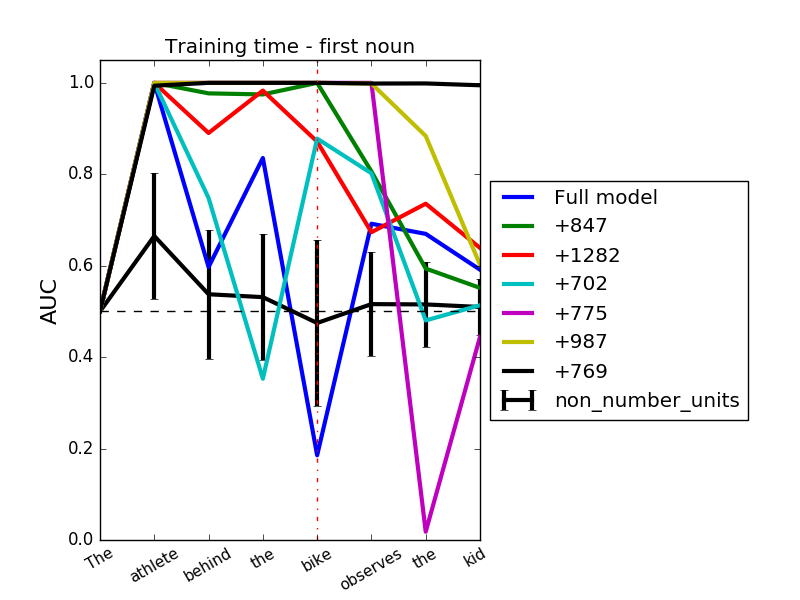
\includegraphics[width=\linewidth]{Figures/Figure3_number_units_GAT.png}
\caption{Generalization across time. To test whether the grammatical number of the first noun can be decoded from units activity at different time points, a linear-SVM was trained on unit activations $h_t$ at the time step of the first noun and then evaluated on all other time points. Area Under of Curve (AUC) values are shown for several cases: decoding from all LSTM units (full-model, black), a single number unit (775, purple; 1282, red...), average across all non-number units (black, error-bars represent standard-deviation). Note that the decoding of first-noun number is significantly higher from number units compared to all other units ($p-value<0.$).}
\end{figure}


\subsubsection{Predicting the verb form}
For long-range dependencies, storing the number of the subject in the cell is necessary for correct prediction in the NA-task (except for cases of mere chance) but is not sufficient. Two more conditions need to be met: (1) the stored number should be output from the cell at the right moment $t_{verb}-1$; and (2) The output from the number unit should increase activations only in units that represent the matching verb form in the output layer. For example, the output from unit 988 should be projected differently to singular and plural verb forms in the output layer, such that it will increase activity only in units representing the singular form. Given that the encoding of singular by unit 988 is with a negative value $C_{t_{verb}-1}<-1$, and therefore $h_{t_{verb}-1}<-1$ (equation 1.x), this means that weights from unit 988 to units in the output layer that correspond to singular forms should be negative too, but not those projecting to plural forms.

\begin{figure*}[ht]
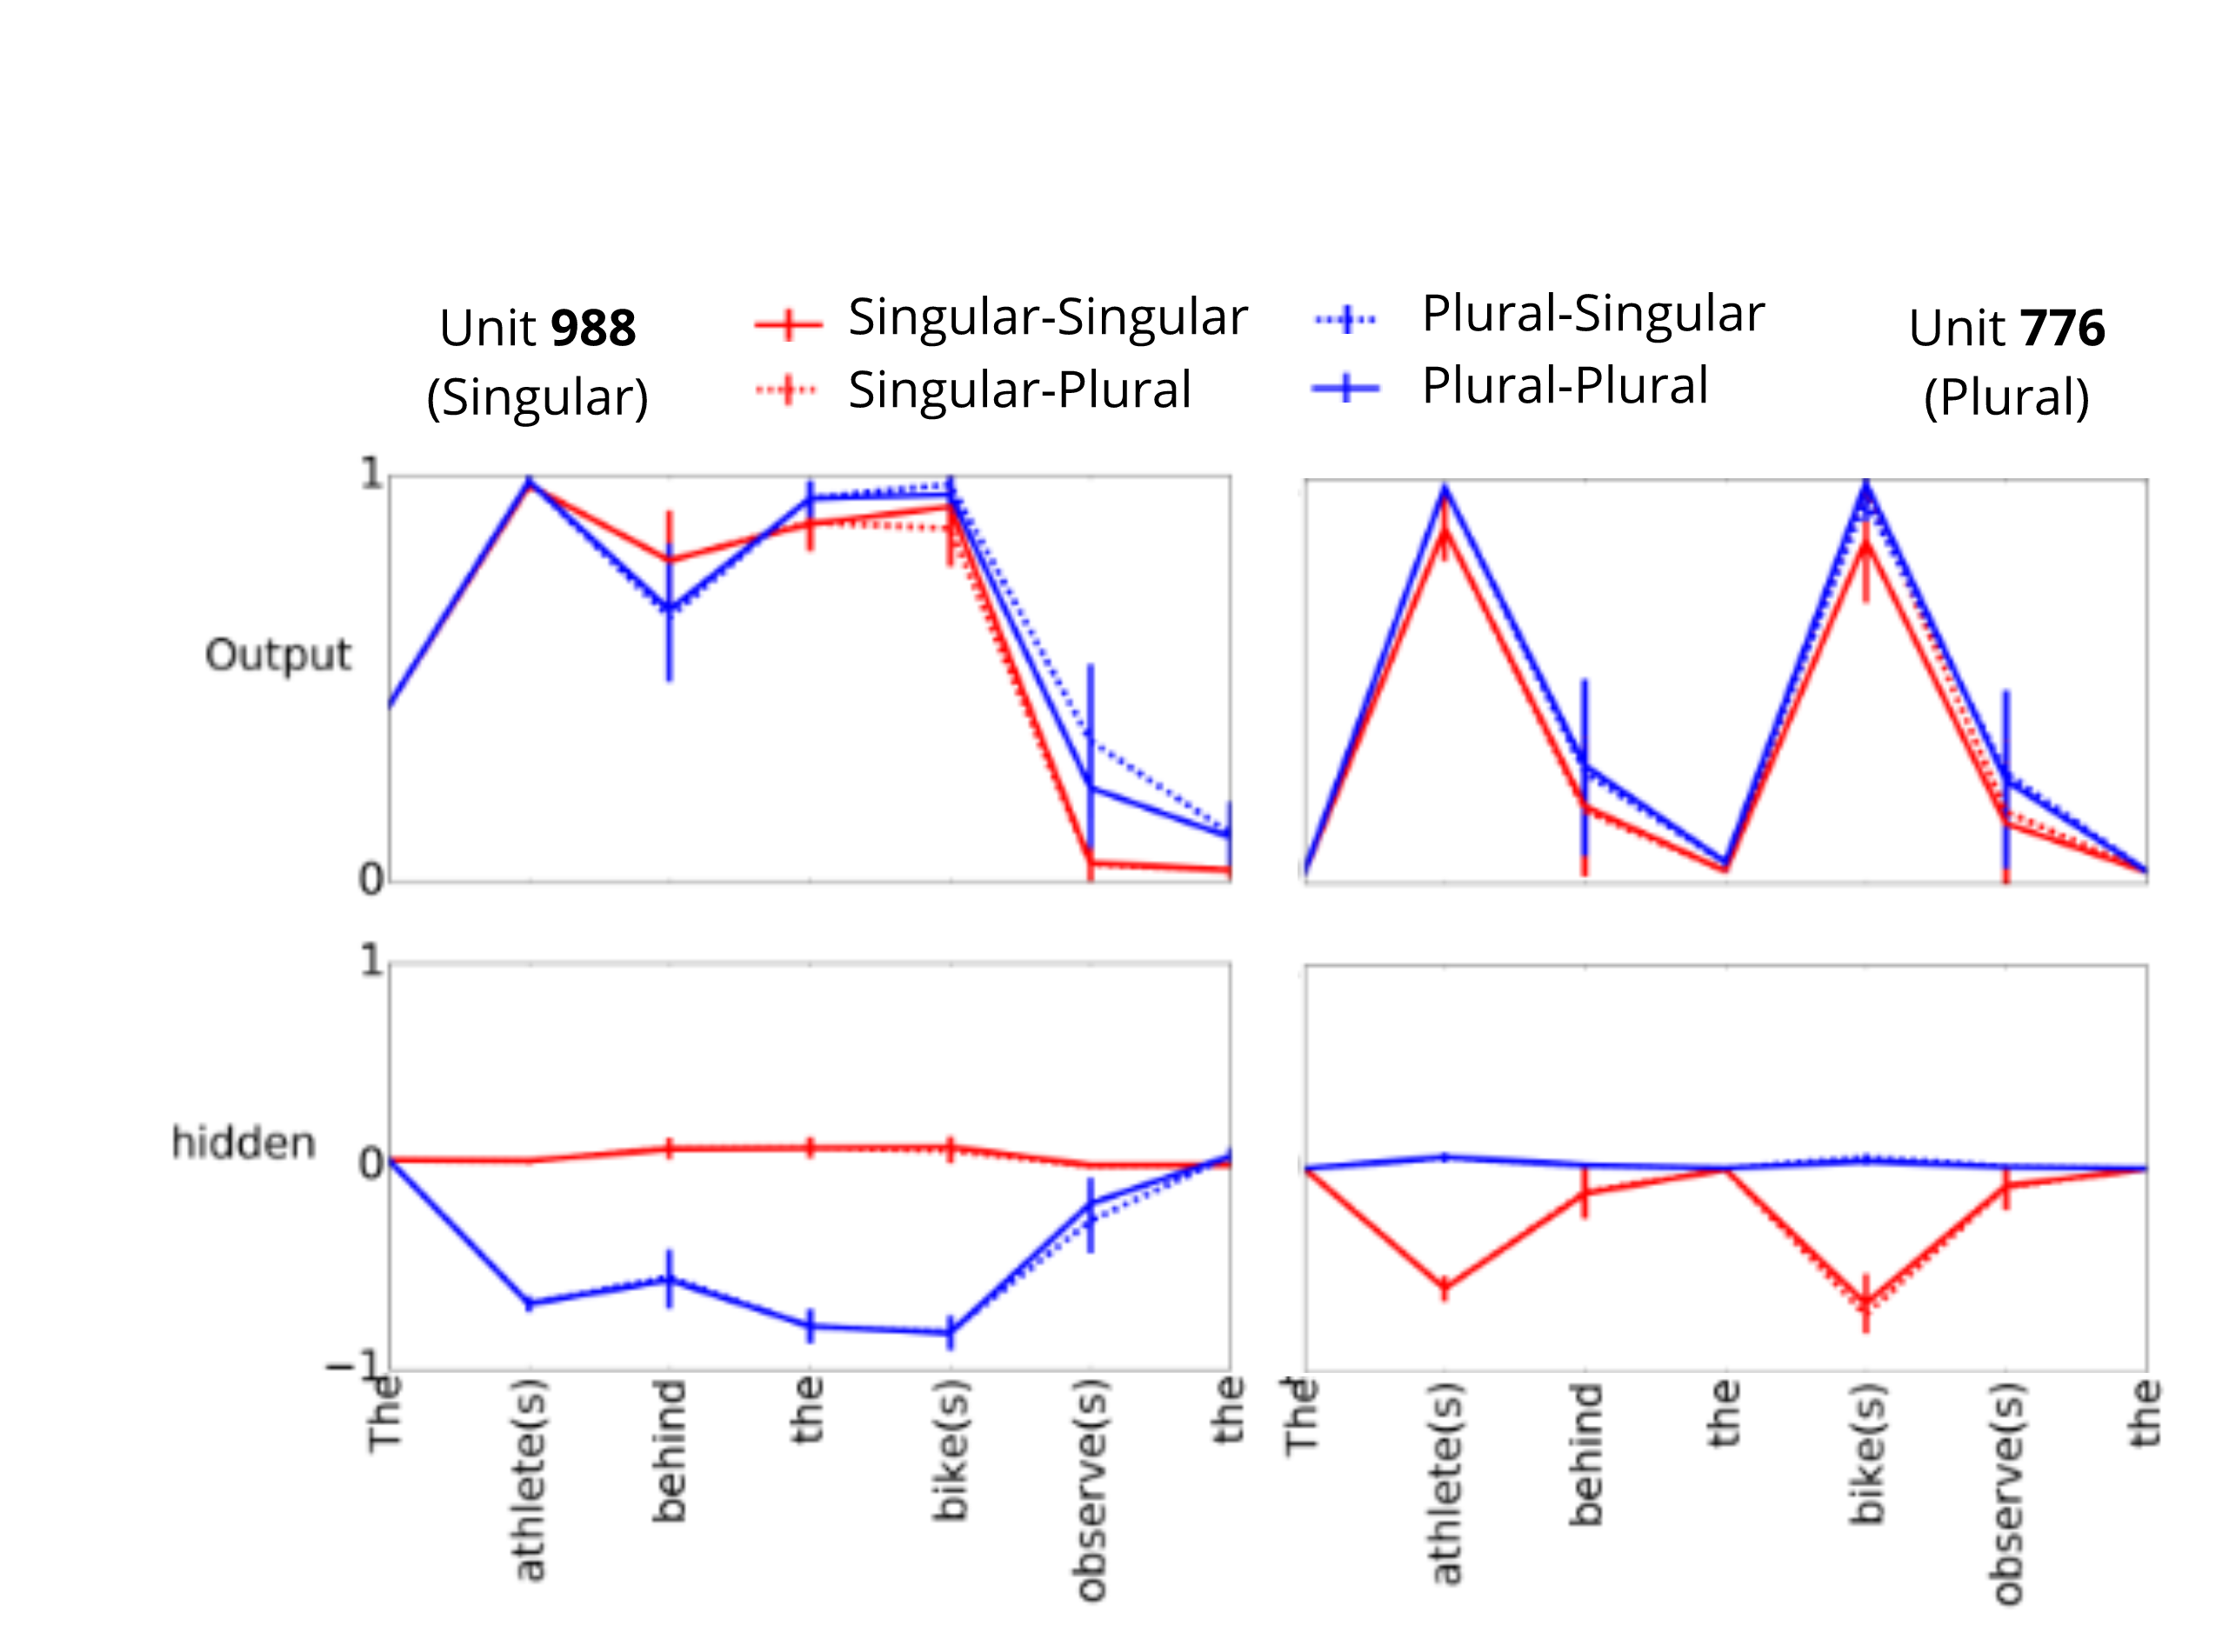
\includegraphics[width=\textwidth]{Figures/Figure3_number_units_775_987_output_hidden.png}
\caption{Hidden and output-gate activations during processing of a sentence with a prepositional phrase between subject and verb. }
\end{figure*}

\begin{figure*}[t]
\centering
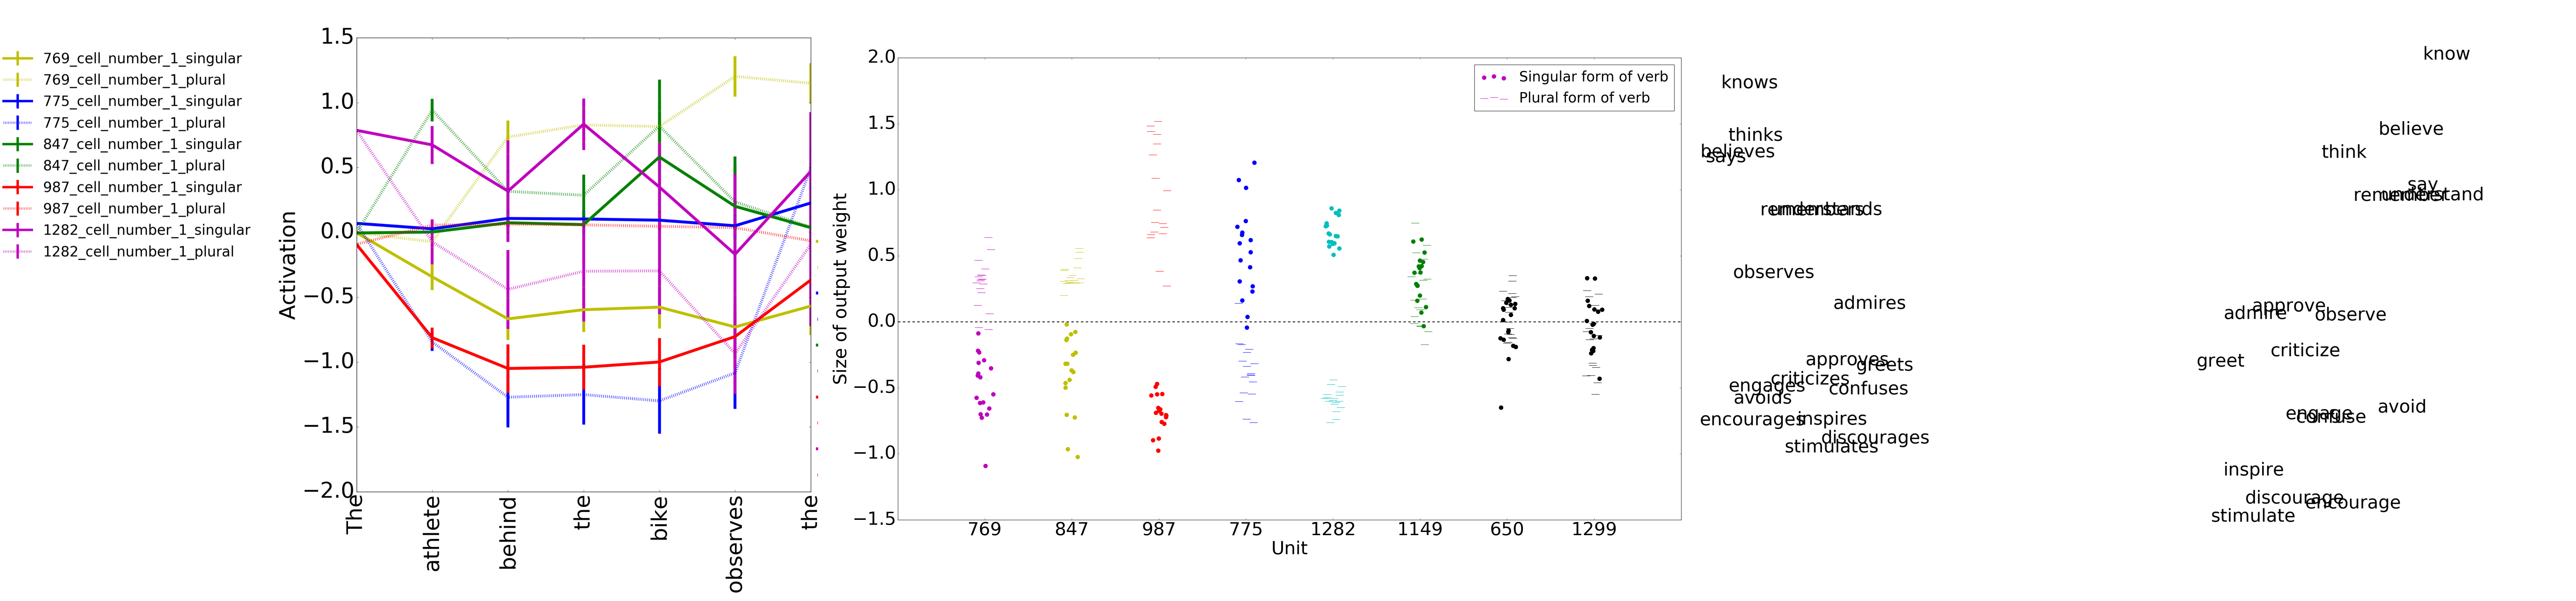
\includegraphics[width=\textwidth]{Figures/Figure4_output_weights.png}
\caption{Connectivity structure to output layer. (A) Output activity $h_t$ of all number units during the processing of a sentence with a PP between subject and verb. (B) Weight values from various units to output layer. Note that only for number units the output weights are clearly separated between singular and plural form of the verb, either positive or negative, compare to the syntax unit (1149) and two non-number units in the second layer. (C) Visualization of 18 verbs in their plural and singular forms (36 words in total) on the plane spanned by the two first principal components of their embeddings by the output weight matrix. A clear separation is observed between the singular and plural form along the first PC.}
\end{figure*}

To see whether number units meet the first condition, figure 4 shows the output-gate and hidden state dynamics of units 988 and 776. Indeed, the output gate opens at $t_{verb}-1$, reaching its almost maximal value (Panels A-B). This ensures that the stored number information is output from the cell and propagates to the output layer via $h_t$ (equation 1.X) at the right moment (Panels C-D). Note also that for both units, output-gate dynamics are quite similar across all four conditions. This may seem sub-optimal, since one may expect that the network would learn to close the output gate for the irrelevant conditions (PS and PP for unit 987 and SS and SP for unit 776). However, as we saw, the cell value for these condition is anyway approximately zero and therefore an open output gate will have the same effect as closed one.

Next, to see whether number units meet the second condition, figure 5 presents the distribution of weight values from all number units and from several other units to 36 units at the output layer - 18 corresponds to verbs in the singular form and 18 to verbs in the plural forms (TODO: extend to more/all verbs in the vocab). Clearly, for number units, weights to singular and plural forms have different values, but for other non-number units, there's no clear structure (panel B). Moreover, the weight values correspond to the encoding of singular/plural in the number unit. For example, weight values from unit 988 to singular forms are indeed negative, and those to plural forms are not. For all other units as well, the sign of $h_{t_{verb}-1}$ corresponds to the sign of the relevant weight values (panels A-B), such that their product is always positive. This ensures that number units increase activations only in the matching units in the output layer.
